
\begin{center}
\Large\textbf{Short-Baseline Neutrino Program}
\end{center}

The discovery that neutrinos undergo oscillation in their flavor, and thus are massive particles, serves as one of the first pieces of evidence for physics beyond the Standard Model (SM) of particle physics. The prevailing description of neutrino oscillations provided by the Pontecorvo-Maki-Nakagawa-Sakata (PMNS) matrix characterizes the flavor change as a result that the neutrino flavor eigenstates ($\nu_{e}, \nu_{\mu}, \nu_{\tau}$) are a linear combination of the neutrino mass eigenstates ($\nu_{1}, \nu_{2}, \nu_{3}$). The rotation from the mass eigenstates to the flavor eigenstates is governed by three angles $\theta_{i,j}$, where $i$ and $j$ correspond to the mass eigenstates with $i < j$, and a phase $\delta$ which determines magnitude of charge-parity (CP) violation within the neutrino sector. Additionally, the flavor change of the neutrinos depends on the ratio neutrino energy and the distance travelled by the neutrino (often referred to as the baseline) as well as the difference in the square of the mass eigenstates $\Delta m_{ji}^{2}$. The exact ordering of the neutrino mass states, known as the mass hierarchy, as well as the size of the CP-violating phase $\delta$ are, as yet, unknown.

Neutrinos produced in the atmosphere \cite{No1, No2, No3}, in nuclear reactors \cite{No4, No5, No6}, in the sun \cite{No7, No8, No9}, as well as in man-made particle accelerators \cite{No10, No11, No12} have been used to study the phenomenon of neutrino oscillations. Going forward, measuring the mass hierarchy and CP-violation can be achieved by studying the appearance of electron neutrinos which oscillate from a beam of muon neutrinos directed at large and precise neutrino detectors. Liquid Argon Time Projection Chambers (LArTPCs) offer fine-grain tracking as well as powerful calorimetry and particle identification capabilities. For these reasons, this detector technology has been chosen for both the study of neutrino oscillations over relatively short baselines ($<1$~km) and long baselines ($>1000$~km).

Into this experimental landscape, there exists a set of series of experimental measurements which suggest that the three-flavor paradigm of neutrino oscillations is incomplete. Two general classes of anomalous observations may point to additional physics beyond the SM  in the neutrino sector.

\begin{itemize}
\item \textbf{The disappearance signal in low energy electron anti-neutrinos from reactor neutrino experiments \cite{No13} \textit{(``Reactor Neutrino Anomaly'')} and Mega-Curie radioactive electron neutrino sources in Gallium \cite{No14, No15} \textit{(``Gallium Anomaly'')}}

\item \textbf{The electron-like excess from muon neutrino (and anti-neutrino) particle accelerators \textit{(``LSND/MiniBooNE Anomaly'')} \cite{No16, No17}}

\end{itemize}

Neither of these anomalies can be accounted for by the standard three-flavor oscillations of the SM and may hint at the existence of additional neutrino states with larger mass difference ($\Delta m_{new}^{2}\geq 0.1 eV^{2}$) which participate in the mixing of the flavour states (referred to as ``sterile neutrinos''). Definitive evidence of the existence of new neutrino states would be a revolutionary discovery with broad implications for both particle physics and cosmology. Moreover, in order for future accelerator based neutrino experiments to disentangle the mass hierarchy and search for CP-violation, the oscillation framework must be concretely known if the appearance of electron neutrinos is to be interpreted properly. 

The conclusive redress of the experimental hints of sterile neutrinos thus becomes high priority for the field of neutrino physics. The Fermilab Short-Baseline Neutrino (SBN) program offers the unique opportunity to definitely address the ``LSND/MiniBooNE'' anomaly. Through the utilization of three liquid argon time projection chambers (LArTPCs) detectors and the decade old and well characterized Booster Neutrino Beam (BNB), the SBN program offers a rich physics program with the ability to perform the most sensitive search to date for the existence of sterile neutrinos at the eV mass-scale.


The Fermilab Short-Baseline Neutrino Program aims to address the electron-like excess seen in the electron neutrino appearance channel. The first experiment to observe this excess was the LSND experiment \cite{No16} at Los Alamos National Laboratory. LSND used a decay-at-rest pion beam to produce muon anti-neutrinos ($\bar{\nu_{\mu}}$) in the energy range between 20-53 MeV and a distance of 30 meters from the liquid scintillator based detector. After five years of running, LSND reported an excess electron like events corresponding to a 3.8$\sigma$ evidence for $\bar{\nu_{\mu}} \rightarrow \bar{\nu_{e}}$ oscillations occurring with a $\Delta m^{2}$ of $\sim 1$eV$^{2}$. This suggests an oscillation beyond the SM three flavor neutrino oscillation which occurs at an $L/E_{\nu} \sim 1$m/MeV.

To test for the appearance of this anomalous oscillation, the MiniBooNE experiment \cite{No17} at Fermilab utilized 700 MeV muon neutrinos produced from the Booster Neutrino Beam at a baseline of 540 meters (thus giving a similar $L/E_{\nu}$ to LSND). MiniBooNE identified muon and electron neutrino interactions by their characteristic Cherenkov rings inside a scintillator detector. As shown in Figure \ref{fig:minibooneExcess}, in ten years of data taking in both neutrino and anti-neutrino running MiniBooNE observed a 3.5$\sigma$ excess in $\nu_{e}$ candidates and a 2.8$\sigma$ excess in $\bar{\nu_{e}}$ candidates. This excess of events observed by MiniBooNE can be due to electrons from $\nu_{e}$ interactions as well as from single photon backgrounds, since these two final states are indistinguishable to the Cherenkov imaging detector.

\begin{figure}[htb]
\centering
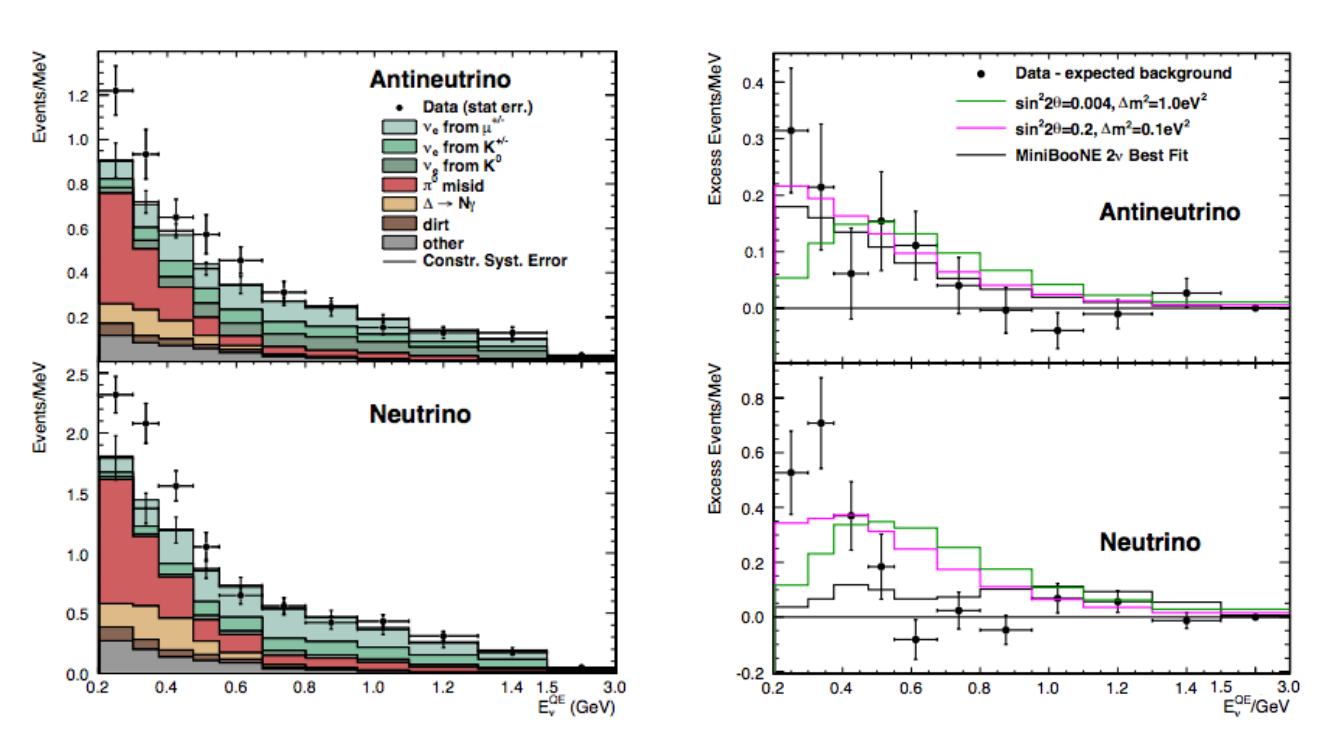
\includegraphics[width=0.85\textwidth]{images/minibooneExcess.png}
\caption[]{Left: Electron anti-neutrino ($\bar{\nu_{e}}$) and neutrino ($\nu_{e}$) candidate events shown with the predicted backgrounds in MiniBooNE. Right: Background subtracted event rates in MiniBooNE as well as different sterile neutrino models overlayed with the data.}
\label{fig:minibooneExcess}
\end{figure}

A common interpretation of this data is to posit the existence of one or more additional sterile neutrino states with masses at or below the eV range. This interpretation requires mixing of the sterile state(s) with both the electron and muon neutrino flavor states. Constraints from sterile mixing from $\nu_{\mu}$ and neutral current disappearance data \cite{No18, No19} leads to significant tension between the $\nu_{e}$ appearance data and the $\nu_{\mu}$ disappearance data. 

To disentangle the open question of how to interpret the LSND/MiniBooNE anomaly, both an excellent neutrino detector technology as well as a robust experimental program is required.  The liquid argon time projection chamber (LArTPC) offers physics capabilities ideally suited for the study of neutrino interactions. By combining millimetre scale tracking capabilities, outstanding calorimetry by having a fully active/sampling detector, and powerful particle identification made by combining the ionization along the particle trajectory (dE/dX) and the topological information, LArTPCs have been chosen to be the premier neutrino detector technology. 

When a neutrino interacts with an atom in the liquid argon multiple final state charged particles as well as electromagnetic objects (such as photons and electrons) can be produced. When the charged particles traverse the liquid argon they produce ionization which drifts along the electric field inside the TPC towards a set of wire planes which are oriented at different angles with respect to each other. As shown schematically in Fig. \ref{fig:LArTPC}, the drifting ions produce an electric signal on the wire planes, which is read out of the detector. By knowing the drift speed of the ions and the timing of the interaction as well as the deposition of charge on the wires a three-dimensional image of the interaction can be reconstructed. The information of the charge deposition as well as the topological information allows for particle identification as well as calorimetric reconstruction. This allows, for example, the ability to disentangle electron initiated electromagnetic showers from photon initiated showers by looking at the displacement in the start of the electromagnetic shower from a primary vertex as well as analysing the energy deposited in the first centimetres of the shower (dE/dX). As shown on the lower right side of Figure \ref{fig:LArTPC} from a measurement done by the ArgoNeuT LArTPC detector \cite{Argoneut}, this provides powerful electron/photon identification capabilities. The resolution of a LArTPC is determined by the spacing of the wires (typically 3-5 millimetres) along with the sampling rate and drift velocity (typically sub-millimetre).

\begin{figure}[htb]
\centering
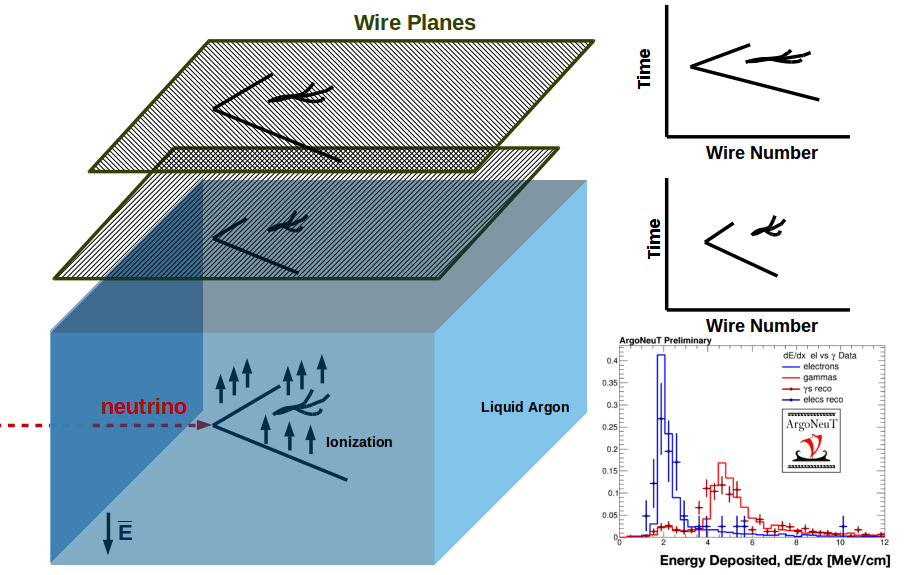
\includegraphics[width=0.55\textwidth]{images/lartpc.png}
\caption[]{Operating principals of LArTPC detectors.}
\label{fig:LArTPC}
\end{figure}

The future short-baseline neutrino programs experimental layout, shown in Fig. \ref{fig:SBNMap}, is designed to include three functionally identical LArTPCs located on-axis in the Booster Neutrino Beam (BNB).  The Short-Baseline Near Detector (SBND) will be a new 112 ton LArTPC and serve as the near detector to the SBN program located 110 meters downstream of the BNB target. SBND will measure the un-oscillated neutrino flux from the BNB and enable searches in both the neutrino appearance and disappearance channels. The MicroBooNE detector is a 89 ton active mass LArTPC located 470 meters downstream of the BNB target (just in front of the MiniBooNE experiment). MicroBooNE serves as the pioneer LArTPC experiment on the BNB and will lay the groundwork for the oscillation analysis. The far detector will utilize the upgraded ICARUS-T600 experiment, previously installed and operated at the Gran Sasso Laboratory, and will be located in a new building 600 meters from the BNB target. ICARUS's large detector mass provides the SBN program with the experimental sensitivity to definitively search for the existence of eV mass-scale sterile neutrinos.

\begin{figure}[htb]
\centering
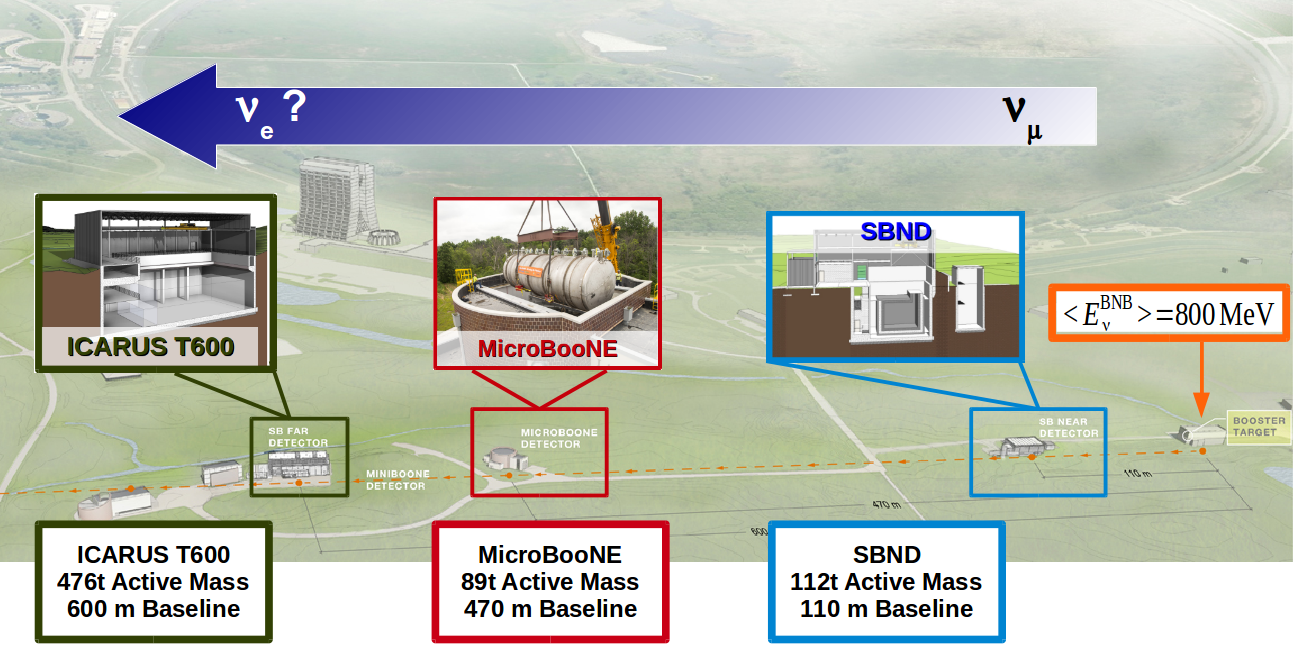
\includegraphics[width=0.75\textwidth]{images/SBNLayout2.png}
\caption[]{Overview of Fermilab's Booster Neutrino Beamline (orange dashed line) campus with the location and description of the three SBN detectors.}
\label{fig:SBNMap}
\end{figure}